\documentclass{sigchi}

% Remove or comment out these two lines for final version
%\toappearbox{\Large Submitted to CHI'13. \\Do not cite, do not circulate.}
\pagenumbering{arabic}% Arabic page numbers for submission. 

% Use \toappear{...} to override the default ACM copyright statement (e.g. for preprints).
\toappear{}

% Load basic packages
\usepackage{balance}  % to better equalize the last page
\usepackage{graphics} % for EPS, load graphicx instead
\usepackage{times}    % comment if you want LaTeX's default font
\usepackage{url}      % llt: nicely formatted URLs
\usepackage{listings}
\usepackage{gensymb}
\usepackage{multirow}
\usepackage{color}

%\usepackage{caption}
%\usepackage{subcaption}

% llt: Define a global style for URLs, rather that the default one
\makeatletter
\def\url@leostyle{%
  \@ifundefined{selectfont}{\def\UrlFont{\sf}}{\def\UrlFont{\small\bf\ttfamily}}}
\makeatother
\urlstyle{leo}


% To make various LaTeX processors do the right thing with page size.
\def\pprw{8.5in}
\def\pprh{11in}
\special{papersize=\pprw,\pprh}
\setlength{\paperwidth}{\pprw}
\setlength{\paperheight}{\pprh}
\setlength{\pdfpagewidth}{\pprw}
\setlength{\pdfpageheight}{\pprh}


% create a shortcut to typeset table headings
\newcommand\tabhead[1]{\small\textbf{#1}}


%************* Andreas Additions
%% Usage: You do not need \begin{enumerate} and \end{enumerate} statements.
%% Just the \squishlist and \squishend statements, and the \items's in between.
%% If you do not want a bulleted list, you can add " [(a)]" after the fist \item,
%% " [(b)]" after the second one, etc, to get a, b, ... bullets...
%% (or 1, 2, 3... can replace the a, b, c...)

\newcommand{\squishlist}{
 \begin{list}{$\bullet$}
 {
  \setlength{\itemsep}{0pt}
  \setlength{\parsep}{0pt}   %3pt
  \setlength{\topsep}{0pt}   %3pt
  \setlength{\partopsep}{0pt}
  \setlength{\leftmargin}{1.5em}
  \setlength{\labelwidth}{1em}
  \setlength{\labelsep}{0.5em} } }

\newcommand{\squishend}{
  \end{list}  }

% Alter some LaTeX defaults for better treatment of figures:
    % See p.105 of "TeX Unbound" for suggested values.
    % See pp. 199-200 of Lamport's "LaTeX" book for details.
    %   General parameterbnos, for ALL pages:
    \renewcommand{\topfraction}{0.9}	% max fraction of floats at top
    \renewcommand{\bottomfraction}{0.8}	% max fraction of floats at bottom
    %   Parameters for TEXT pages (not float pages):
    \setcounter{topnumber}{2}
    \setcounter{bottomnumber}{2}
    \setcounter{totalnumber}{4}     % 2 may work better
    \setcounter{dbltopnumber}{2}    % for 2-column pages
    \renewcommand{\dbltopfraction}{0.9}	% fit big float above 2-col. text
    \renewcommand{\textfraction}{0.07}	% allow minimal text w. figs
    %   Parameters for FLOAT pages (not text pages):
    \renewcommand{\floatpagefraction}{0.7}	% require fuller float pages
	% N.B.: floatpagefraction MUST be less than topfraction !!
    \renewcommand{\dblfloatpagefraction}{0.7}	% require fuller float pages

	% remember to use [htp] or [htpb] for placement


% Adds a space between the text and the [T]op \hline
% Must use the \T *within* a cell, not right after the \hline
\newcommand\T{\rule{0pt}{2.5ex}}%{3.1ex}}

% Adds a space between the text and the [B]ottom \hline
% Must use the \B *within* a cell, not right after the \hline
\newcommand\B{\rule[-1ex]{0pt}{0pt}}%[-1.7ex]{0pt}{0pt}}

% Enable grayed-out text environments, like {\graytext foo}:
\definecolor{gray}{RGB}{163,163,163}
\newenvironment{graytext}{\color{gray}}{\ignorespacesafterend}

%\setlength{\belowcaptionskip}{-3pt}

%************* End Andreas Additions


% Make sure hyperref comes last of your loaded packages, 
% to give it a fighting chance of not being over-written, 
% since its job is to redefine many LaTeX commands.
\usepackage[pdftex]{hyperref}
\hypersetup{
pdftitle={SIGCHI Conference Proceedings Format},
pdfauthor={LaTeX},
pdfkeywords={SIGCHI, proceedings, archival format},
bookmarksnumbered,
pdfstartview={FitH},
colorlinks,
citecolor=black,
filecolor=black,
linkcolor=black,
urlcolor=black,
breaklinks=true,
}
\renewcommand{\baselinestretch}{0.98}

% End of preamble. Here it comes the document.
\begin{document}

\title{EchoTree: Engaged Conversation when Capabilities are Limited}

% Note that submissions are blind, so author information should be omitted


\numberofauthors{2}
\author{
  \alignauthor Andreas Paepcke, Sanjay Kairam\\
    \affaddr{Stanford University, Stanford, CA.}\\
    \email{paepcke/skairam@cs.stanford.edu}
    }

% \author{
%  \parbox[t]{18.0cm}{\centering 
%    {\em Andreas Paepcke\**}, 
%    {\em Caroline Pantofaru\**\**}, 
%    {\em Dirk Thomas\**\**}, 
%    {\em Austin Hendrix\**\**}, 
%    {\em Sharon Marzouk\**\**},
%    {\em Sarah Elliot\**\**}}\\
%  \\
%  \parbox[t]{5.0cm}{\centering
%         \**Stanford University\\
%         353 Serra Mall\\
%         Stanford, CA 94305\\
% 	paepcke@cs.stanford.edu}\\
%  \\
%  \parbox[t]{10.0cm}{\centering
%     	\**\**Willow Garage\\
% 	68 Willow Road\\
% 	Menlo Park, CA 94025\\
%        \{pantofaru,dthomas,ahendrix,smarzouk,selliott@willowgarage.com\}}
% }

% Teaser figure can go here
%\teaser{
%  \centering
%  \includegraphics{Figure1}
%  \caption{Teaser Image}
%  \label{fig:teaser}
%}

\maketitle

\begin{abstract}
We describe the collaborative use of word tree visualizations, {\em
  EchoTree}s, to facilitate face-to-face, and remote communication
with speech and movement impaired individuals. EchoTree is designed to
bridge the inevitable conversational dead space while the impaired
person uses assistive technologies to generate written, or
artificially spoken sentences. Visualizations that guess multiple
conversational directions in which the impaired person might be headed
keep conversation partners engaged. Partners may call out
possibilities, which the impaired person can confirm or
dismiss. Correct guesses accelerate conversational progress. EchoTrees
are browser based and interactive. Multiple parties may view, and
interact with the same stream of EchoTrees from desktops, tablets, or
smartphones. The application may also be used for collaborative,
geographically remote story telling games, whose participants may, or
may not be pysically impaired. We describe our implementation, and
provide preliminary measurements of how effectively EchoTrees predict
conversation flow for one particular underlying set of text
materials. 
  \end{abstract}

\keywords{assistive technology; prolonged engagement; collaborative conversation; story telling, game}

\category{H.5.2}{Information Interfaces And Presentation}{User Interfaces - Interaction styles}

\terms{Human Factors; Design}


\tolerance=400

%\newcommand{\degree}{$^\circ$}

\section{Introduction}
We collaborate with a motion and speech impaired individual, Henry,
who enjoys conversing. Henry's speech impairment is
complete. Quadriplegia, while severely limiting, does allow Henry to
move his head in affirmation or negation. His hand can operate a mouse
button. One of his communication modes is via a text-to-speech system
({\em tts}). A camera mounted on top of his laptop tracks a confetti
sized white dot pasted on the lower left of his glasses. The resulting
cursor control allows Henry to hunt down the keys of an onscreen
keyboard. On a very good day the resulting speed is 15 words per
minute. The tts produces sound once a sentence is complete. Uttering
words as Henry types them would work, but this approach makes it
difficult for listeners to track the very slowly evolving sentences in
their minds. Poor tts performance for some words would additionally
impede comprehension, which is supported by context when a full
sentence is pronounced in a flow.

This slow communication channel results in very frustrating
experiences during gatherings like parties. A guest will make a remark
to Henry, who will go to work on an answer. To the conversation
partner Henry looks frozen, peering at his laptop screen whose back
surface reveals nothing to the expectant partner. Often the potential
conversation partner wanders off bewildered before Henry can finish
his response sentence.

One improvement would be to install a second display on the backside
of Henry's laptop. Inexpensive, USB based options are available. This
option would at least allow a listener to understand that information
is forthcoming. The option does not help as much as possible in
keeping the listener(s) actively involved in the conversation. 

In an attempt to ameliorate the situation further we developed
EchoTree. EchoTree is a distributed, collaborative word
tree. Figure~\ref{fig:echoTree} shows an example.
\begin{figure}
   \centering
   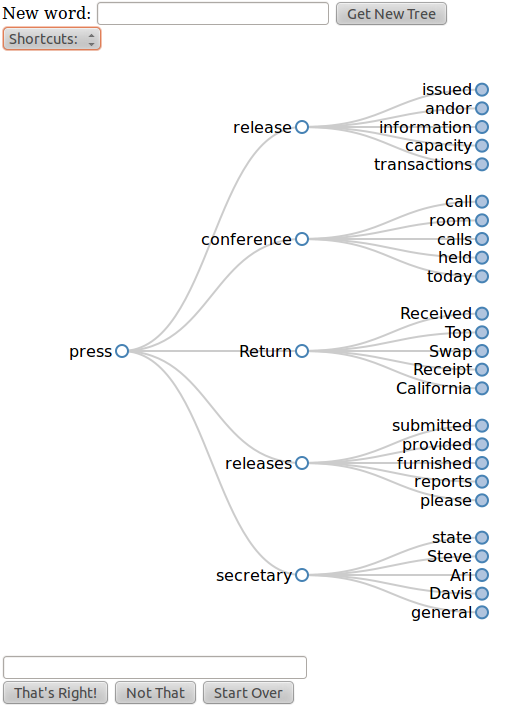
\includegraphics[width=0.6\columnwidth]{Figs/echoTreeScreenshot.png}
   \caption{Screenshot of an EchoTree browser.}
   \label{fig:echoTree}
\end{figure}
Henry, of course, stands for many individuals with similar
impairments. 
\section{User Experience}
EchoTrees are browser applications that can be viewed anywhere, by
multiple users. For example, the secondary display facing a
conversation partner in the option discussed earlier could show an
EchoTree. Alternatively, a conversation partner's smartphone could
{\em tune in} to Henry's EchoTree. After describing the interface and
some of its interaction affordances we explain how an EchoTree can be
related to Henry's response activity.

The word on the left most node of Figure~\ref{fig:echoTree} is called
the {\em root word}. In case of the Figure the root word is {\em
  press}. Links connect the root node to the five `most frequently
following' other words.  `Most frequently following' is measured in
the context of an underlying text collection. We will discuss this
dependency later.

Each of the word followers is connected to the five words that most
frequently follow {\em it} in the underlying texts. Following, for
example, the top branches in Figure~\ref{fig:echoTree} we find the
sequence ${press, release, issued}$.

In the current implementation anyone viewing an EchoTree on their
device may click or tap on one of the circles. In response all the
displayed EchoTrees are {\em re-rooted}: the selected word becomes the
root of a new tree. All follow words are recomputed, and a new tree is
displayed on all browsers. Figure~\ref{fig:todayTree} shows the result
of clicking on the word {\em today} in Figure~\ref{fig:echoTree}'s
tree. 
\begin{figure}
   \centering
   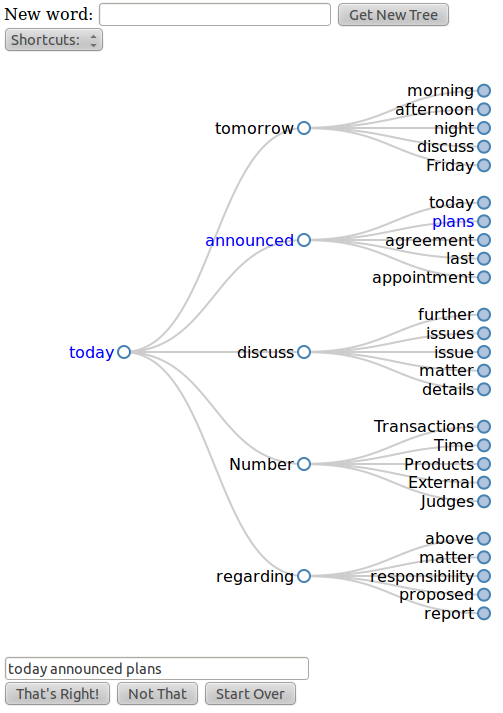
\includegraphics[width=0.6\columnwidth]{Figs/echoTreeRootToday.png}
   \caption{EchoTree re-rooted in `today'. Blue words were user
     selected, adding them to the sentence box.}
   \label{fig:todayTree}
\end{figure}
Alternatively, one may type a new word into the text box at the top,
and click on the button {\em Get New Tree}. This action again creates
a new tree, rooted at the new word, and displayed everywhere.

Instead of clicking/tapping on a circle, participants may target one
of the words with a click or tap. This action causes two changes in
the display. First, the targeted word turns blue, and second, the word
is added to the text field at the bottom of the display. This field is
called the {\em sentence box}. Figure~\ref{fig:todayTree} shows the
result of clicking on {\em today}, then {\em announced}, and finally
{\em plans}.

The EchoTree facility can be used for a number of purposes. In the
context of Henry interacting in a conversation, the facility may be
used as follows. 

\subsection{Collaborative Conversing}
As Henry types words, EchoTrees in the browsers of all tuned in
listeners will evolve, the latest word always serving as root. Any
word that Henry completes is additionally appended to the sentence
box. Listeners, meanwhile may actively think ahead and guess where
Henry might be headed. After scanning the current EchoTree they can
call out possibilities. If Henry hears a hit, he can click on the {\em
  That's Right} button, or nod. After a successful guess Henry can
continue, skipping one of more words.

Of course, if Henry notices a word that matches his intention, he can
click on that word in the EchoTree himself. If the content of the
sentence box is hopelessly wrong, the {\em Start Over} button will
clear the box, and turn off all blue (i.e. selected) words in the
EchoTree. 

The underlying machinery will exclude a fixed set of stopwords in the
EchoTrees. This filtering helps maximize use of the limited tree node
real-estate. Sometimes participants may wish to enrich sentences with
fill words. The pull-down menu below the {\em New word} field
satisfies that need (Figure~\ref{fig:shortcuts}). Selecting any of
these words will enter them in the sentence box. Again, in the current
implementation this addition appears in all views of the EchoTree.
\begin{figure}
   \centering
   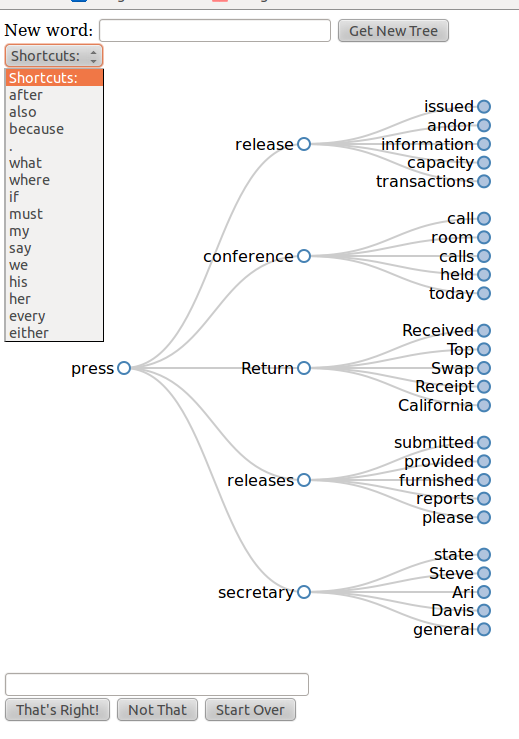
\includegraphics[width=0.4\columnwidth]{Figs/echoTreePulldownSnapshotSmall.png}
   \caption{Shortcut words are available as fillers for the sentence
     box. These stopwords will not occur in EchoTrees.}
   \label{fig:shortcuts}
\end{figure}
Note that the use of EchoTrees for collaborative conversation is not
limited to face-to-face situations, like parties. Communication
with Henry via the telephone are also an option. The remote
participant tunes into Henry's EchoTrees, and offers guesses over the
phone. Since Henry nodding assent is not an option in this scenario,
the {\em Not That} button can serve as a negative response.

\subsection{Story Telling Game}
Instead of supporting a directed conversational thread, EchoTrees can
serve as a collaborative story telling facility. Geographically
distributed players click on words in a starting EchoTree,
collaboratively adding words to the sentence box. Various rules might
govern the process. Participants might take turns, or work at speed
without turn taking limitations. Re-rooting might earn a demerit,
while opening new possibilities.

This application is accessible to disabled and non-impaired
participants. Again, the goal is mutual engagement. Appropriate rules
in this scenario can provide satisfying interaction even in the
presence of speed limitations.

\subsection{Architecture}
Figure~\ref{fig:arch} shows how the EchoTree system is
constructed. 
\begin{figure}
   \centering
   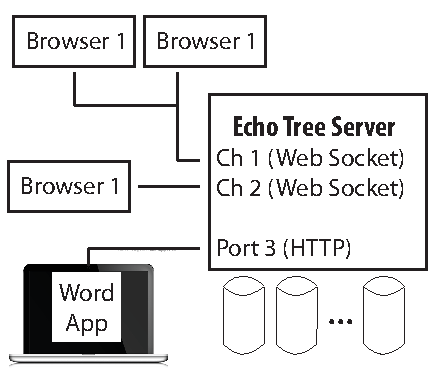
\includegraphics[width=0.5\columnwidth]{Figs/echoTreeArch.pdf}
   \caption{EchoTree architecture. Channels are implemented as
     WebSocket ports. Browsers tune in to different EchoTree channels.}
   \label{fig:arch}
\end{figure}
Central, or distributed EchoTree servers each manage some
number of distinct EchoTree channels. All facilities described above
operated on one channel. All shared EchoTree views are refreshed, and
request re-rooting on one channel. The server computes the trees,
given a root word.

Multiple, unrelated EchoTree sequences may be served by a single
server, using different ports. In Figure~\ref{fig:arch}
Brower~3 is separated from Browsers one and two, which share all
EchoTree transmissions.

Browsers communicate with EchoTree servers via WebSocket connections,
which are bi-directional. This bidirectionality enables the re-rooting
requests from browsers back to the server.

Figure~\ref{fig:arch} also shows an HTTP port family. These ports can
push new words to the echo server, triggering the multicast of a new
EchoTree to all browsers on the respective channel. These HTTP
connections are simpler than the more versatile WebSocket
connections. They are provided for easy connection with word entry
support applications on Henry's machine. For example, Henry uses an
application that offers word completions as he types a word. The HTTP
method of pushing words to the EchoTree server can be attached to this
application. This method allows Henry to focus on typing in his usual
environment, and not being forced to interact with a browser's {\em
  New Word} entry to push a new word (and consequently a new
EchoTree).

Figure~\ref{fig:arch} shows a series of databases with word pair
frequencies that are the basis for the generation of the trees. The
word pairs are word collocation statistics, or {\em bigrams}.  Each
database holds lists of triples: a word, a follower word, and a
frequency count. These bigram counts may originate from any text
collection. Given a root word, EchoTree, like other word tree
visualizations, recursively finds follow-on words, which are chosen by
maximum frequency.

The trees of the above figures are based on bigrams from the Enron
collection ~\cite{enron}. In the following section we examine some
aspects of this underlying collection, which strongly influence the
induced EchoTrees.

\section{Effectiveness Experiment}
EchoTrees could be effective along several dimensions. Each dimension
implies a different evaluation method. 1.Conversation acceleration
through word prediction, 2.Conversation acceleration by conveying
intent, 3. Encouragement through bi-- or multilateral engagement, and
4. Fun.
%% \squishlist
%% \item[1.] Conversation acceleration through word prediction.
%% \item[2.] Conversation acceleration by conveying intent.
%% \item[3.] Encouragement through bi- or multilateral engagement.
%% \item[4.] Fun
%% \squishend
We measured the first item in an experiment, which we will describe in
this section. This dimension works by accurately predicting the next
word the current utterance originator is planning to type.

The second dimension in the above list contributes not through
prediction, but by helping the listener imagine indirectly where the
typist is heading. The inspiration might for example arise from
associations with words that occur in the EchoTree, though those
literal word might not even feature in the typist's plan.

The third dimension simply helps keep the conversation partners
connected. All listeners can at least observe progress, and maybe
anticipate a chance to complete a sentence soon.

The final dimension, finally, contributes by raising enjoyment in the
interaction. This element is most obvious in the story telling
scenario. All dimensions can contribute cumulatively, and are worthy
of evaluation. An examination of the word prediction power is an
important start. 

\subsection{Prediction Measurement Setup}
Like all word prediction, EchoTrees depend for their predictive power
on the match between the word source and the underlying frequency
data. We tested and compared two such pairings in an experiment
%shown in Table~\ref{tab:conditions}.
%###################################
%% \begin{table}{\scriptsize
%%     \begin{tabular}{|r|c|c|}
%%          % \T and \B would not work if it is placed here (needs to go inside cell)
%%         \hline
%%         ~                & {\bf Enron Collection} \T \B & {\graytext\bf Google Bigrams} \\ \hline
%%         {\bf Non-Enron} \T & ~    & ~  {\graytext\em Planned}     \\ 
%%         {\bf Enron EmpX} \B & ~   & ~  {\graytext\em Planned}     \\
%%         \hline
%%     \end{tabular}
%%     }
%%     \caption{Experiment matching utterance originators with
%%       word prediction source(s). Gray entry shows future work, and
%%       exemplifies how suitability of additional collections will be evaluated.}
%%     \label{tab:conditions}
%% \end{table}
%###################################
Our findings are preliminary. For our experiment we used the 2.6GB
Enron collection of emails produced within the Enron corporation. It
comprises 48,900 emails. After stopword removal our bigram database
from these emails contains 3,881,632 entries.

In order to measure the sensitivity of EchoTrees to the underlying
bigram source we used 40 emails that Henry sent to a mailing list. The
emails contained a total of 2246 words, including lengthy quoted
emails to which Henry was replying. These emails were thus paired with
a bigram source that was unrelated to any of Henry's content.

For comparison we then randomly picked one of the Enron employees
who is represented in the Enron collection: EnronEmpX. From that
employee's emails we again picked 40, which in total contained 7435
words. 

For each word in both email sets we generated EchoTrees of the type
shown in the above figures. We measured {\em success}, {\em outOfSeq},
and the tree depths at which successful matches occurred. Given a word
from the emails, a {\em success} is the presence of that email's next
word anywhere in the tree. An {\em outOfSeq} event occurs when a tree
does not contain the email's immediately following word, but does
contain a word later in the same sentence. The measure {\em
  netSuccess} for one sentence is the sum of {\em success} and {\em
  outOfSeq} as a percentage of the respective sentence's length.
\subsection{Results}
Figure~\ref{fig:netSuccess} shows the average {\em netSuccess} for
both the Enron originating emails, and the emails not related to Enron
(i.e. Henry's messages). Coloration shows the contribution of {\em
  outOfSeq} to the overall result.
\begin{figure}
   \centering
   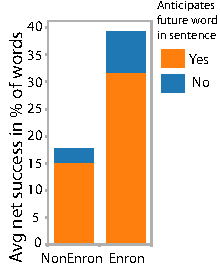
\includegraphics{Figs/relativeNetSuccessBarGraphCleanedSmall.pdf}
   \caption{Using own corporation's collection is advantageous, though
     still far from perfect. Many of the EchoTrees forshadowed words
     in the future of a sentence (shaded areas).}
   \label{fig:netSuccess}
\end{figure}
Prediction success was 15.2\% for EnronEmpX, and 4.2\$ for
NonEnron. Beyond this binary measure, we examined whether the {\em
  degree} of {\em netSuccess} within sentences differed significantly
in the two cases. For this purpose we excluded sentences with complete
failure. After a $log$ transformation to assure normality of the {\em
  netSuccess} measure's distribution, a T-test yielded $t(319)=-4.1,
p<.001$.
\section{Discussion}
The Enron collection is very biased towards the energy business, and
is thus suboptimal as a source for prediction in unrelated
domains. The collection's superior performance for EnronEmpX would
suggest to go one step further, and use an individual's own email as
the bigram source. 

However, an application that requires access to a user's content is
more cumbersome, and less secure to use than a more general facility.
Unfortunately, for motion impaired email users this downside is
exacerbated because their text collections tend to be sparse.
Their messages are short.

Another option is a learning component, which would over time adjust
bigram weights to each user. Both, computational linguistics, and
machine learning algorithms can help.

Given the significant number of {\em outOfSeq} hits, we will add
a {\em word stash} element to our UI design. This element will collect
any words in an EchoTree that users indicate to be relevant for their
immediately upcoming communication plan.

The {\em optimal} text source for prediction will likely depend not just on
a user, but on that user's context when generating words whose
followers are to be predicted. For this reason the EchoTree
architecture (Figure~\ref{fig:arch}) anticipates multiple bigram
sources that can be switched dynamically.

\section{Related Work}
EchoTree draws on prior work in reducing text input demands for
impaired users through the use of language modeling and prediction
techniques. Existing systems such as Humsher~\cite{Polacek2011}, for
example, have adapted letter-based text entry systems designed for
able-bodied users to significantly accelerate text entry for users
with severe motor impairments.

Trnka, et al. motivate the use of word-based prediction, finding that
the increased typing rates offered by {\em n-gram}-based word
prediction can offset the additional cognitive load they may
introduce~\cite{Trnka2009}. Roark, et al. identified how human
guessing and n-gram prediction models can complement each other in
important and useful ways~\cite{Roark2011}. By incorporating the
conversation partner and word-prediction model into a single
conversational loop, EchoTree builds on and extends these insights
from prior work.

EchoTree's design draws heavily on the visual 'keyword-in-context'
technique embodied in the Word Tree by Wattenberg and
Viegas~\cite{wattenberg2008}. EchoTree adapts this technique from its
original purpose of analyzing text corpora to the new problem of
collaborative text generation. The use of visual metaphors, direct
interaction, and output-as-input techniques allow for tight coupling
between the conversation participants and the information
display~\cite{Ahlberg1994}. The sentence box and confirmation loop
further afford the process of {\em grounding}, enabling tighter
coupling between the conversation partners themselves as they
negotiate the evolving sentence together.

\section{Future Work and Conclusion}
EchoTree leaves room for many user experience improvements,
optimizations, and effectiveness measurements. For example, we plan to
examine how well the Google bigram statistics over scanned books, and
the American National Corpus \cite{anc} can serve as a driver.

Short of precise word prediction, the EchoTree scenario makes it
likely that the visualizations would convey conversational {\em
  intention}. If an EchoTree makes conversation partners guess the
intended direction, then much weaker performance in literal word
prediction is acceptable.

Our strongest hope for EchoTree is that it will help blur the
distinction between conversation partners of varying physical
abilities. 

\section{Acknowledgments}
Thank you to Henry Evans for patient testing, and encouragment of
crazy ideas. And: we are grateful to Sean Kandel for his JavaScript
prowess, and willingness to apply it.
%-------------------


% Balancing columns in a ref list is a bit of a pain because you
% either use a hack like flushend or balance, or manually insert
% a column break.  http://www.tex.ac.uk/cgi-bin/texfaq2html?label=balance
% multicols doesn't work because we're already in two-column mode,
% and flushend isn't awesome, so I choose balance.  See this
% for more info: http://cs.brown.edu/system/software/latex/doc/balance.pdf
%
% Note that in a perfect world balance wants to be in the first
% column of the last page.
%
% If balance doesn't work for you, you can remove that and
% hard-code a column break into the bbl file right before you
% submit:
%
% http://stackoverflow.com/questions/2149854/how-to-manually-equalize-columns-
% in-an-ieee-paper-if-using-bibtex
%
% Or, just remove \balance and give up on balancing the last page.
%
\balance

% If you want to use smaller typesetting for the reference list,
% uncomment the following line:
% \small
\bibliographystyle{acm-sigchi}
\scriptsize{\bibliography{echoTree}}
\end{document}
